\chapter{Best Practices}
\label{ch:bp}

In dit hoofdstuk zijn alle gehanteerde best practices terug te vinden van de twee applicaties. Algemene best practices zijn het gebruik van Github en daarbinnen werken met Git Flow. Zo hebben we voor alle belangrijke use cases een aparte branch aangemaakt die pas op de master branch mogen na dat iemand anders de pull request reviewed.

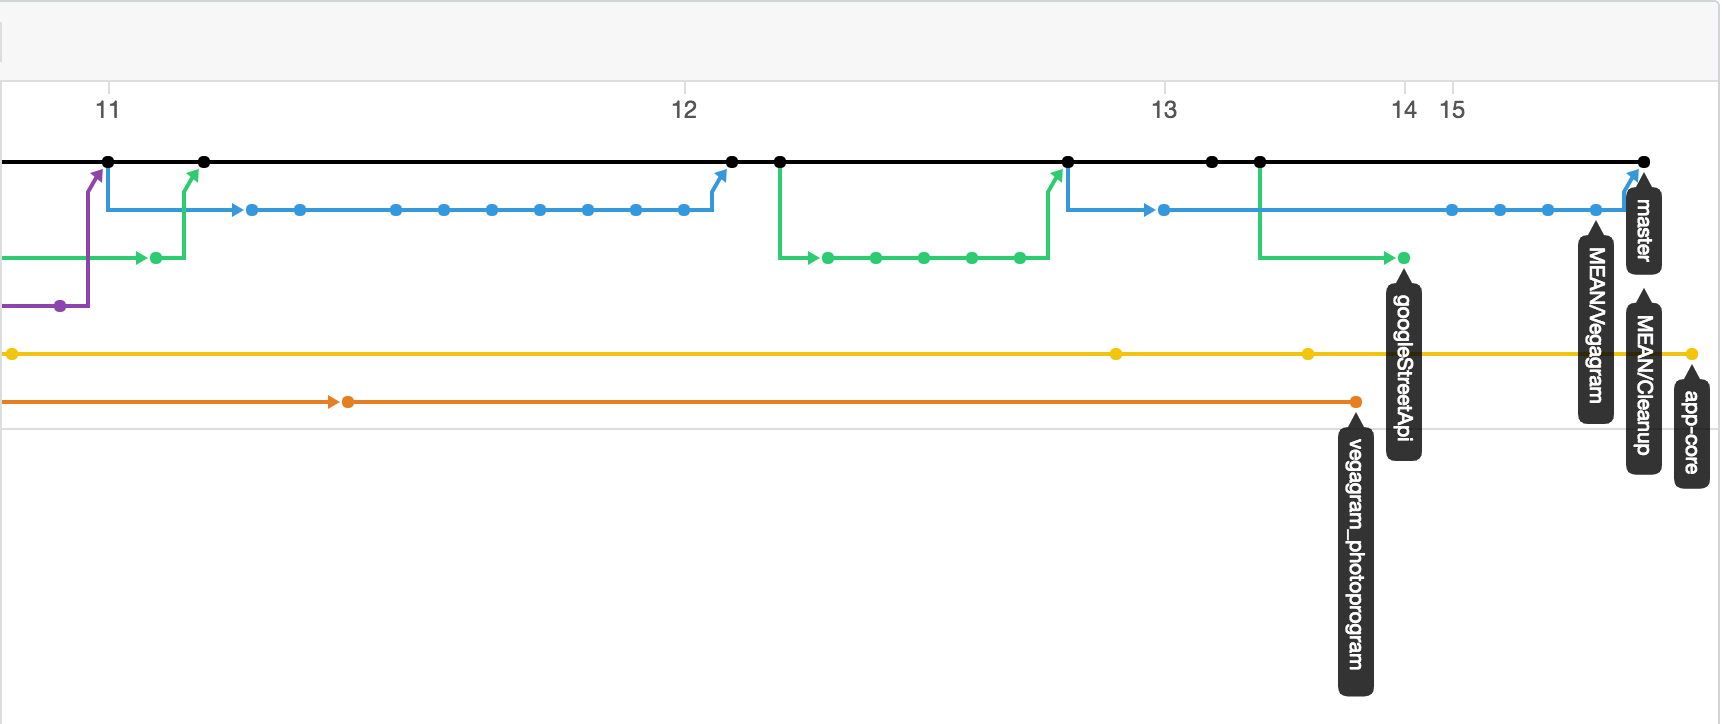
\includegraphics[width=15cm]{img/branches.png}

Als men surft naar:
https://github.com/BramVannevel/eva2017groepH4/pulls?utf8=\%E2\%9C\%93\&q=
is\%3Apr\%20is\%3Aclosed\%20
zijn ook alle gesloten pull requests zichtbaar.

En andere best practice, wat ook aangehaald zal worden in het hoofdstuk met betrekking tot de analyse is onze communicatie. Voor teamcommunicatie hebben we gebruik gemaakt van de handige tool Slack. Hiermee kunnen teams eenvoudig communiceren met elkaar. Slack staat ook toe dat men andere tools integreerd. Zo hebben wij Trello geïntegreerd in Slack waardoor iedereen kan zien wanneer een ticket klaar is. Ook GitHub werd toegevoegd zodat daar direct duidelijk is wanneer een pull request of code review gevraagd werd door een teamlid.

De Trello updates zagen er zo uit

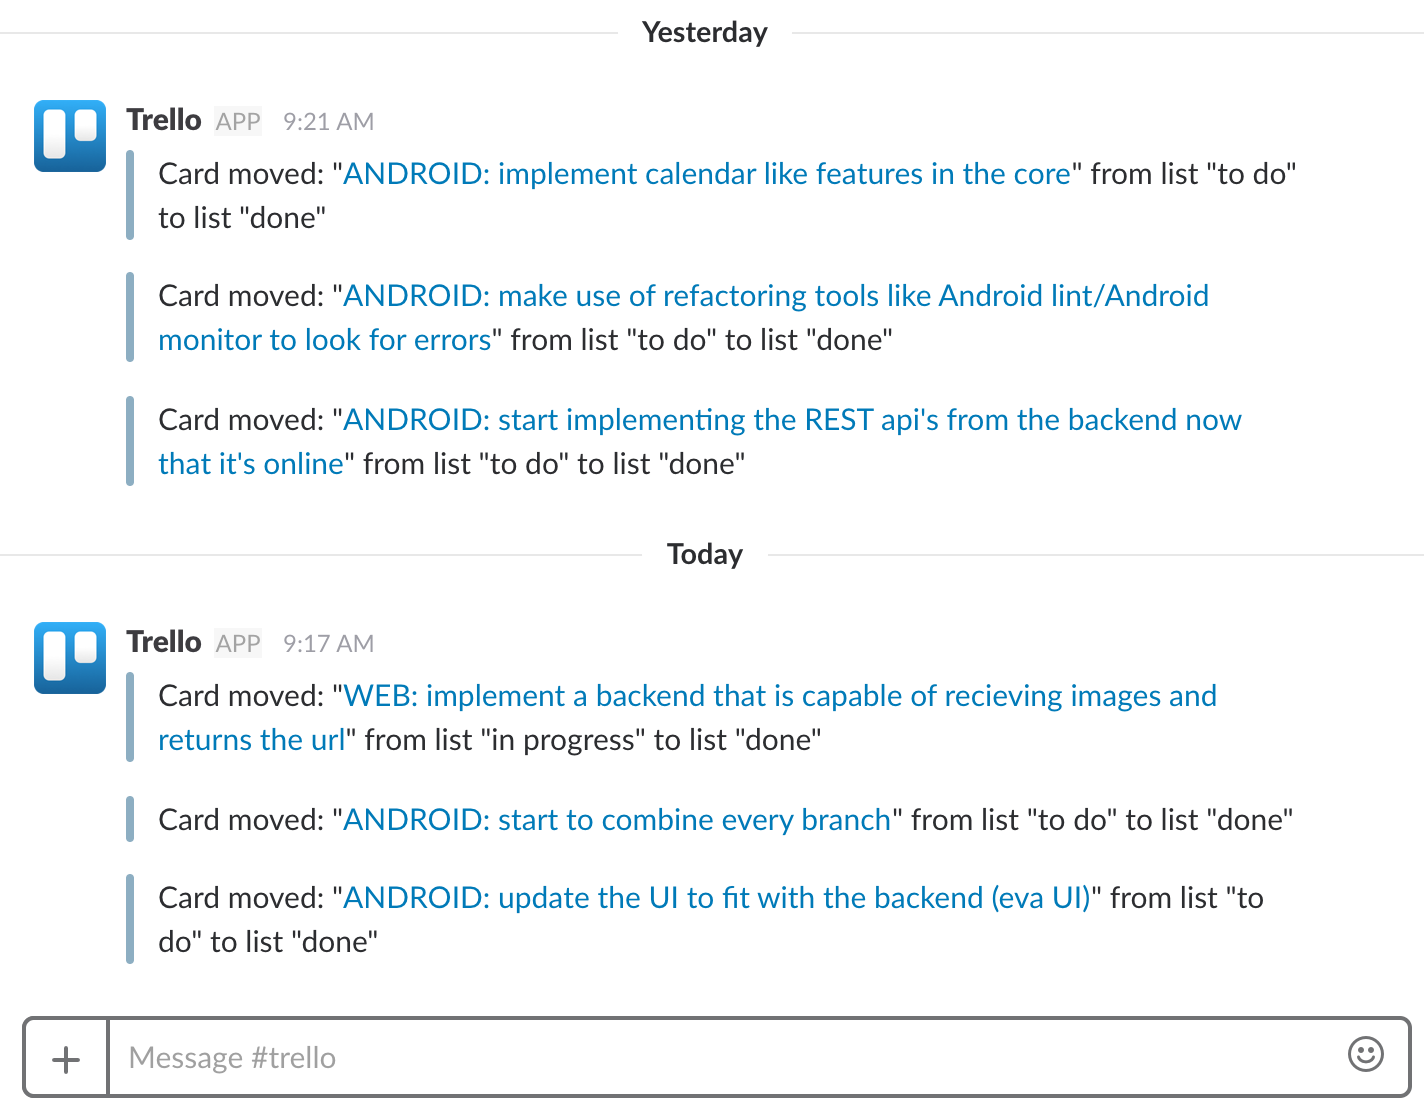
\includegraphics[width=15cm]{img/slack.png}

Binnen slack is het ook eenvoudig om de statistieken te bekijken, zoals hieronder getoond.

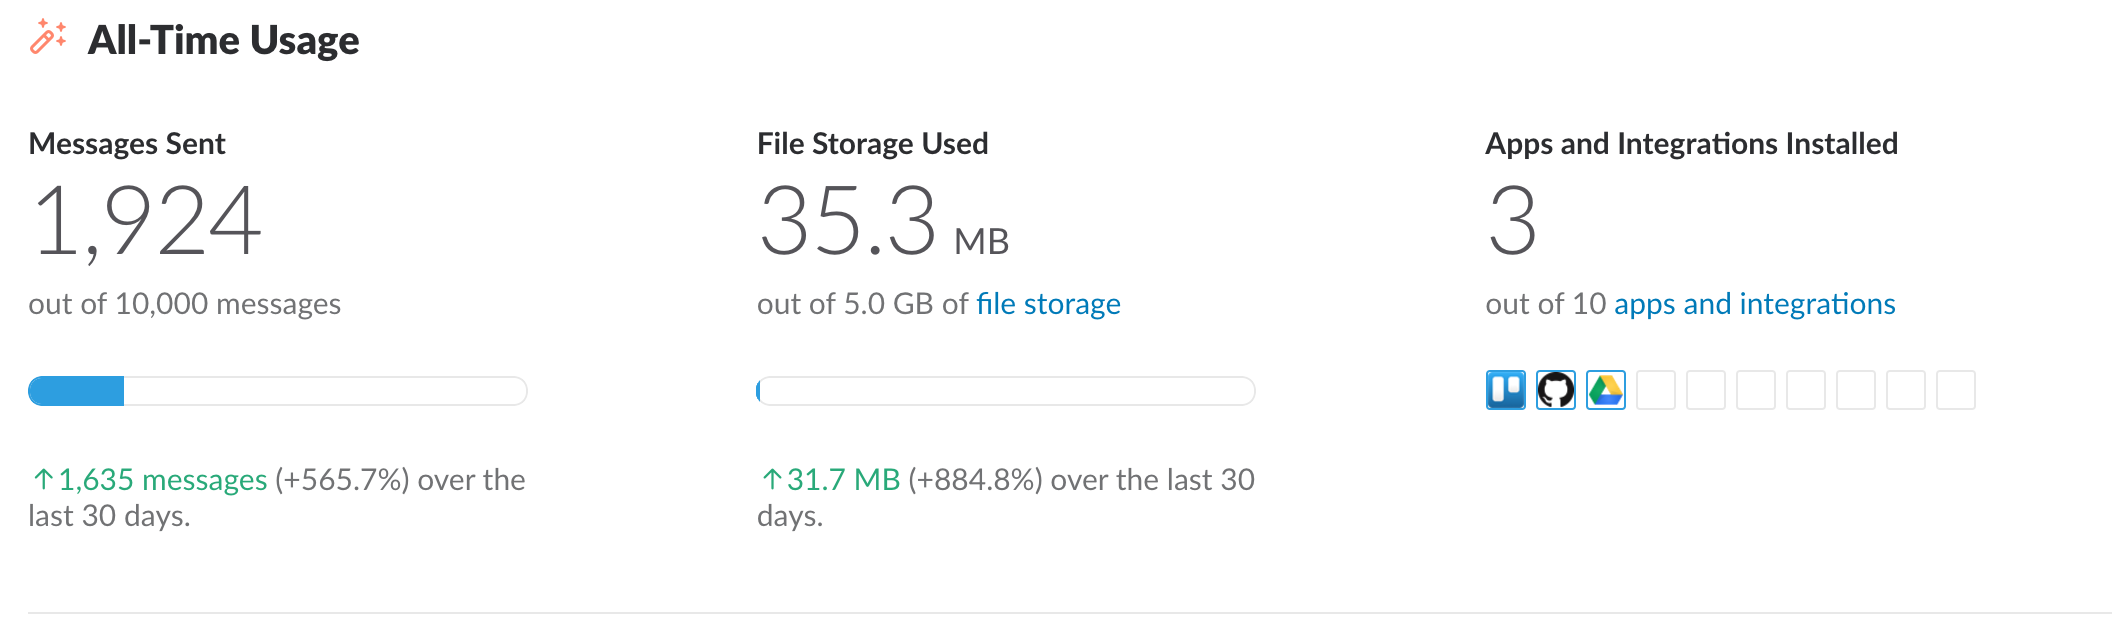
\includegraphics[width=15cm]{img/slack_integrations.png}

Als laatste hebben we ook de scrum en agile principes gerespecteerd en hebben we een scrummaster aangewezen en in iteraties van één week gewerkt per sprint. Dit is allemaal terug te vinden onder het hoofdstuk met betrekking tot de Analyse.


\section{Android}
Binnen Android zijn er veel best practices en normen die gehanteerd en gevolgd kunnen worden om een goede Look and Feel te garanderen voor een app. Zoals het material design. Ook op implementatieniveau zijn er belangrijke verschillen tussen een goede, onderhoudbare app en een minder goede. 

De belangrijkste best practice die achter de schermen gebeurt, maar direct vertaalt naar de user experience van de app is dat alles dat netwerk en databank gerelateerd is asynchroon gebeurt. Voor de netwerk communicatie bekomen we dit door gebruik te maken van OkHttp, Retrofit en RXJava. Dit zorgt voor een asynchrone manier van data ophalen dat perfect in overeenkomst is met de Android Lifecycle van activities en fragments. De reden dat RXJava hierin betrokken wordt, kan het best aangetoond worden aan de hand van onderstaand voorbeeld. 

Als een gebruiker de app opstart en nieuwe uitdagingen ophaalt kan het zijn dat, bijvoorbeeld door het roteren van het apparaat of het openen van een andere applicatie, de activity die de data wil opvragen er niet meer is. Indien men enkel Retrofit gebruikt zal dit leiden tot een crash. Want de asynchrone bevraging zal de data proberen afleveren aan een activity die er niet meer is. Door gebruik te maken van RXJava kunnen we effectief werken met een observer pattern en kunnen activities hun subscriben op data, en als ze destroyed worden unsubscriben zodat de data weet dat ze daar niet naar toe kunnen. Ook heeft RXJava enkele methodes, zoals defer, die kunnen ingeschakeld worden om enkel de data te beginnen opvragen als het effectief nodig is.

Een tweede best practice is het gebruik van een SQLite databank om de gebruiker zijn vooruitgang bij te houden. Zo kan de gebruiker ook offline zijn challenges en vooruitgang bekijken.

Als derde code best practice wordt ook gebruik gemaakt van instancebundles om opgehaalde data in de activity te houden zolang die niet destroyed is. Zo hoeft de applicatie niet altijd een netwerk call te maken als de gebruiker verwisselt van schermen om daarna terug te keren naar het eerste scherm. Zoals bijvoorbeeld het geval is in de Vegagram activity om de posts bij te houden.

Ook wordt veel gebruik gemaakt van fragments zodat een tablet versie ook een makkelijk te implementeren mogelijkheid is. Verder rond UI wordt ook veel gebruik gemaakt van de (relatief) nieuwe ConstraintLayout omdat deze veel performanter is dan RelativeLayout en aanverwanten. Voor het tonen van lijsten gebruikt de applicatie Recyclerviews met als rij een cardview, die opgevuld worden aan de hand van het viewholder patroon. Voor creaties met meerdere mogelijkheden gebaseerd op een input werden meerdere factories geïmplementeerd.

een overzicht van gebruikte patterns:
\begin{itemize}
	\item Factory pattern
	\item Observer pattern
	\item Viewholder pattern
	\item Singleton pattern
	\item Builder pattern
\end{itemize}

kleine, en niet gebruikersgevoelige info wordt opgeslaan in de shared preferences zodat die snel en eenvoudig overal aanspreekbaar zijn, bijvoorbeeld een Json Web Token (jwt). 

Zoals eerder aangehaald is de mappenstructuur ook zeer intuïtief en makkelijk uitbreidbaar bijvoorbeeld om bepaalde classes terug te vinden. Een meer algemene code best practice is ook dat de code zo geschreven is dat ze makkelijk uitbreidbaar en aanpasbaar is. Door middel van factories, interfaces en design keuzes. Een voorbeeld van zo een design keuze is het startscherm. Hier zien we vier knoppen die in een grid terug te vinden zijn. Initieel werden die geïmplementeerd door middel van een TableLayout en dan vier maal hard gecodeerde knoppen in cardviews toegevoegd, maar na een pull request en analyse kwamen we tot het besef dat dit niet uitbreidbaar nog onderhoudbaar is. In de app wordt nu gebruik gemaakt van een Recyclerview met dynamisch gegenereerde knoppen gebaseerd op één klasse die ze kent. Stel dat EVA nog functionaliteit wenst toe te voegen of extra knoppen kan dit op één plaats en wordt alles overal aangepast.


Een laatste best practice is het feit dat er gebruik gemaakt werd van de resource bundles. Zo zitten alle strings in de string resource alsook alle colors. De gebruikte iconen binnen de applicatie zijn afkomstig van de vectors die terug te vinden zijn en gratis te gebruiken, onder de Apache Licentie. Dit heeft als voordeel dat elk icoon op elke smartphone er goed uit ziet.

Binnen Android werken we ook veel met afbeeldingen, zoals de afbeeldingen die kunnen getrokken worden en de Vegagram Posts die getoond worden van andere gebruikers die publiek zijn. De best practice, zoals beschreven in onderstaande sectie, bestaat uit het feit dat geen afbeeldingen direct mee komen via de GET calls. We slaan de afbeeldingen op op de server, en sturen een url naar de afbeelding mee met de call. Dit bespaart tijd (lengte van de duur van de call), geheugen en data van de gebruiker zijn toestel. Daarna kunnen de foto's ingelezen worden via libraries zoals Glide of Picasso en zo door.

\section{MEAN}

Ook voor het webgedeelte werd rekening gehouden met best practices. Zo wordt er gebruik gemaakt van Webpack om alle statische resource bestanden te bundelen. Om de CSS overzichtelijk te houden werd er gebruik gemaakt van Sass. Binnen angular werd de functionaliteit netjes opgesplitst aan de hand van controllers, factories en services en wordt voor de navigatie tussen de verschillende paginas gebruik gemaakt van angular-ui-router. 
Om de verschillende endpoints voor de netwerkoperaties overzichtelijk te houden, werd er gebruik gemaakt van een 
individuele module met constanten. Ook met security werd rekening gehouden. Zo maakt het webgedeelte gebruik van een JSON Web Token 
voor de authenticatie en worden alle wachtwoorden eerst gehashed alvorens ze worden gepersisteerd.
Om ervoor te zorgen dat enkel admins kunnen inloggen in de webapplicatie, werd gebruik gemaakt van gebruikersrollen.
Enkel gebruikers met de rol 'admin' kunnen succesvol inloggen in het webgedeelte. Ook wie van buitenaf (bijvoorbeeld via postman) een 
HTTP request stuurt naar een endpoint dat enkel bedoeld is voor admins, krijgt indien hij dit doet met een account met de rol 'user' een
403 Unauthorized response. Op deze manier blijven alle gegevens binnen het bereik van de juiste personen.

Voor het mongoDB gedeelte hebben we, door dat we werken met afbeeldingen, ook rekening gehouden met de persistentie en efficiëntie van de databank. Zo worden afbeeldingen via een POST als binary opgeslagen op de server zelf (via /uploads/MulterNaamVanDeAfbeelding). Enkel de link naar de afbeelding wordt opgeslaan in de databank. Op die manier blijft deze snel en responsief. En is het mogelij om de afbeeldingen te laden door gewoon de link te gebruiken. Dit heeft ook als voordeel dat er geen afbeeldingen mee gestuurd worden via de GET call van de vegagram posts. Dat zou te veel data verbruiken en te veel geheugen consumeren van de Android applicatie.